\chapter{Improving Southern Ocean boundary layer cloud parametrisation in the general circulation model HadGEM3-GA7.1/UM11.4}

\section*{Abstract}

Southern Ocean cloud biases and the resulting shortwave and longwave radiation
biases are a longstanding problem in the HadGEM3 general circulation model. We use one month of high-resolution summertime
Southern Ocean voyage ceilometer and radiosonde observations collected on the Aotearoa/New Zealand research vessel Tangaroa in February--March
2018 in the Ross Sea region
and a nudged run of HadGEM3-GA7.1/UM11.4 to
evaluate the impact of modifications in the convection and boundary layer
schemes on cloud representation in a case study approach. We use the recently-developed Automatic Lidar and Ceilometer Framework (ALCF) to assess and improve the representation of stratocumulus (Sc) cloud,
currently strongly underestimated in the model. We show that a two- and three-layer cloud
profiles of cumulus (Cu) below Sc corresponding to local thermodynamic levels were a common occurrence, where
the Cu cloud base height coincides with lifting condensation level (LCL)
and the Sc cloud height coincides with the neutral buoyancy level of a dry and moist air
parcels lifted from the surface. While the thermodynamic levels were simulated
well by the model, not enough moisture was transported to the top of the boundary layer.
By increasing surface moisture flux and convective mass flux in the model we improve the
Sc cloud simulation, but we show that a lack of vertical moisture transport
across LCL from the surface layer to the zone of convective mass flux is a likely limiting factor.
We show that the modifications had a positive impact on the Southern Ocean and
global radiation balance of up to 5 \unit{Wm^{-2}} in zonal average over this limited time period.

\section{Introduction}

Cloud biases in general circulation models (GCMs) are a long-standing problem
\citep{vignesh2020}. Correct cloud representation in GCMs is critical due
to its strong effect on the planetary albedo and longwave emissivity as well as
being a latent heat source and the source of precipitation. Cloud biases are
currently a key contributor to the error in the present-day Earth
radiation balance simulation in GCMs \citep{li2013}. Clouds in contemporary
GCMs are parametrised by subgrid-scale parametrisation schemes. Cloud typically vary at scales much lower
than the resolution of the models, which is on the order of 10--100 km. Therefore, many of the physical
processes responsible for cloud formation and removal such as convection and cloud microphysics are not resolved at the
model resolution and have to be parametrised. These parametrisations come with
large uncertainties. An alternative to such schemes are cloud resolving models
(CRM), which operate at a much higher spatial resolution (on the order of 1 km)
\citep{guichard2017,satoh2019}.
At present it is unfeasible to use these models for long-term climate
projections due to computational demands. Therefore, a continued improvement of
existing cloud schemes is needed.

Cloud parametrisation in GCMs is traditionally improved by intercomparing with
observations such as the ISCCP satellite-based cloud dataset \citep{rossow1991}
or more recently the CloudSat-CALIPSO datasets
\citep{stephens2002,winker2003}. By accomplishing a good match with past and
present observations of cloud it is assumed that cloud representation in
simulations of future climate will be reasonable. However, the physical
processes responsible for any cloud bias are not necessarily obvious from an
intercomparison, which may be due to processes outside of the cloud
parametrisation scheme \citep{morcrette2010}. The presence of compensating
errors can make the model perform worse when only one of the errors is
corrected \citep{hourdin2017}.

Here, we focus on the Southern Ocean (SO) cloud parametrisation in the
Global Atmosphere 7.1 (GA7.1)/Unified Model 11.4 (UM11.4) component of the
Hadley Centre Global Environment Model 3 (HadGEM3) \citep{walters2019},
with the aim of improving the
simulation of boundary layer (BL) cloud. The GA7.1 model is based the  UK Met Office
Unified Model (UM), which is also used for operational numerical weather
prediction (NWP). As shown by \cite{kuma2019}, cloud
fraction in a previous version of the model is underestimated in the SO by about 6--8\%, with low cloud below 1 km
and fog particularly underestimated compared to ship-based ceilometer
observations. \cite{schuddeboom2019} and \cite{kuma2019} noted that 55$^\circ$S
is a clear dividing latitude between positive and negative shortwave (SW) radiation
bias in HadGEM3-GA7.1 and that the positive vs. negative bias is linked to
near-surface air temperature, with negative bias strongly associated with
close to zero near-surface air temperature. Therefore, we expect that
near-surface temperature and sea surface temperature (SST) have a significant role in the cloud bias,
potentially by destabilisation of the relatively cold Antarctic air in the surface
layer by near-zero SST. \cite{loveridge2019} also implicated quiescent conditions in the
SO BL cloud bias in GA7.0. Considering these past findings, here we focus
on BL cloud south of 60$^\circ$S, which we will call here
"high-latitude SO", as opposed to "low-latitude SO" north of 60$^\circ$S.

The UM parametrises clouds using a prognostic scheme PC2
\citep{wilson2008a,wilson2008b}, in which the cloud condensate (liquid and ice)
and cloud fraction are prognostic variables defined on 85 vertical model levels
on every grid cell. The prognostic variables can be advected with the
large-scale flow, and this is fin contrast with earlier schemes which were purely
diagnostic \citep{smith1990}, and based on the assumption that any
supersaturation is turned into cloud condensate \citep{jakob2000}. Cloud
condensate and cloud fraction originating in the convection scheme are injected
into the condensate and cloud fraction of the cloud scheme and thus become
prognostic. Schemes which
used prognostic condensate and diagnostic cloud fraction also exist
\citep{sundqvist1978,sundqvist1989}.

An improvement in the SO cloud representation in the MRI-ESM2 GCM has recently been
reported by \cite{kawai2019}. This model uses a cloud scheme based on
\cite{tiedtke1993}. This is the same as the basis of the PC2 scheme, although both
schemes likely contain many modifications of the original. Therefore, it may be
possible to gain insight from this study for the improvement of PC2 in this
region. They reported that their updated stratocumulus (Sc) scheme resulted in about
10\% increase in SO cloud cover and 10 Wm$^{-2}$ increase in top of atmosphere
(TOA) outgoing SW radiation over the SO, reducing the model bias.

This paper is outlined as follows.
In Sect. \ref{sec:methods} we briefly describe the TAN1802 voyage dataset,
the HadGEM3-GA7.1/UM11.4, and the lidar processing and simulator framework ALCF.
In Sect. \ref{sec:parametrisations} we describe the
relevant characteristics of the cloud-related parametrisation schemes in the UM
and an experimental run of the HadGEM3-GA7.1/UM11.4. Finally, in Sect.
\ref{sec:results} we contrast the results
of the experimental run with the control run and observations.

\section{Methods}
\label{sec:methods}

\subsection{TAN1802}

In our analysis we use ceilometer, radiosonde and AWS data collected on the TAN1802 voyage
of R/V Tangaroa in the Ross Sea. The data were collected
between 16 February and 15 March 2018 UTC (inclusive), when the ship was south of
60$^\circ$S. The deployed ceilometer was a Lufft CHM 15k operating at an
infrared wavelength of 1064 nm vertically between the surface and 15 km above
sea level (ASL). We process the raw backscatter profiles with
the ALCF (Sect. \ref{sec:alcf}). In addition, we use radiosonde profiles
sampled during the voyage at approximately 1--3 times daily intervals
using the iMet-1 ABx radiosondes. Near-surface air temperature, relative humidity (RH) and SST were
sampled continuously during the voyage. The TAN8102
voyage atmospheric measurements also described in greater detail by
\cite{kuma2019} and \cite{hartery2020}. The track of the voyage
is shown in Fig. \ref{fig:map}.

\subsection{HadGEM3-GA7.1/UM11.4}

The GA7.1 model is the atmospheric component of the HadGEM3 GCM.
Specifically, it is based on the UK Met Office Unified Model (UM), which is an
atmospheric model used for both NWP and GCM purposes in global and regional
configurations. HadGEM3 is a proprietary model developed by the UK Met Office
and partner organisations in a number of countries. We analyse data from a relatively
recent version UM11.4 released on 21 Jun 2019. The experiments were performed on the NeSI
supercomputer in Wellington, Aotearoa/New Zealand \citep{williams2016}.
The horizontal grid scale of the model is N96,
corresponding to about 100$\times$140 km grid cells at
60$^\circ$S. The time step of the model is 20 minutes. We use
instantaneous 3-dimensional atmospheric fields exported from the model at each time
step and process these with the ALCF (Sect. \ref{sec:alcf}) to obtain simulated
lidar data corresponding to the TAN1802 voyage. We use the UM11.4 in a "nudged"
configuration, in which SST and sea ice concentration are prescribed from
the HadISST dataset \citep{rayner2003} and atmospheric fields are nudged to the
ERA-Interim reanalysis \citep{dee2011}. In this configuration the large-scale
dynamics is effectively prescribed from observations, while parametrised fields
such as cloud are still the result of the model's physics. Here, we analyse
two simulations produced by the UM11.4: (1) an unmodified control run "UM11.4cnt"
and (2) an experimental run "UM11.4ext" (Sect. \ref{sec:experimental-run}).
The parametrisations in the HadGEM3-GA7.1/UM11.4 are described in Sect. \ref{sec:parametrisations}.

\subsection{ALCF}
\label{sec:alcf}

The Automatic Lidar and Ceilometer Framework (ALCF) \citep{kuma2020} is a lidar
simulator and lidar processing tool, based on the Cloud
Feedback and Model Intercomparison Project (CFMIP) Observation Simulator Package
(COSP) \citep{bodas-salcedo2011}. We use ALCF to process the ceilometer
observations collected on TAN1802 and to simulate backscatter profiles based
on the UM11.4 model output.

\section{Parametrisations}
\label{sec:parametrisations}

The UM11.4 relies on parametrisation of subgrid-scale processes,
which cannot be represented by the atmospheric dynamics on the relatively
coarse horizontal grid of the model. The parametrisations directly affecting cloud
are the convection, boundary layer and large-scale cloud (PC2) schemes
and the related parametrisation of surface fluxes in the surface component of
HadGEM3 called the Joint UK Land Environment Simulator (JULES) \citep{best2011,clark2011}. The formation
and destruction of cloud is therefore an interplay of a relatively large number
of parametrised processes. It is typically not obvious from model
evaluation studies which process is responsible for a bias in cloud occurrence
or TOA radiation balance. The parametrisations outlined above operate independently
on each individual horizontal grid cell of the model.
Table \ref{tab:parametrisations} summarises the cloud-related
parametrisation schemes, described in a greater detail below with a specific
focus on aspects important to BL cloud.

\subsection{Large-scale cloud scheme (PC2)}

The PC2 scheme is based on an earlier work of \cite{tiedtke1993}. The motivation to
develop a new scheme was to allow for detrainment of convection into cloud
fraction and break diagnostic link between cloud fraction and condensate
\citep{umdp030}. The scheme contains a separate treatment of large-scale (stratiform) and
convective cloud, both of which contribute to the cloud condensate and cloud
fraction by detraining moisture and condensate. Moisture in the PC2 scheme
within a grid cell is assumed to have a probability distribution function around
the grid mean, parametrised by a critical RH \citep{gregory2002}.
Therefore, supersaturation within the grid cell can occur before mean
RH reaches 100\%. This probability density function (PDF) is defined explicitly in PC2, in
contrast with previous schemes \citep{tiedtke1993}, which assumed an implicit
PDF \citep{wilson2008a}.
The PC2 calculates the evolution of condensate and cloud fraction by summing the
contributions of a number of sources and sinks in each model time step:
advection,  boundary layer (Sect. \ref{sec:bl-scheme}),
convection (Sect. \ref{sec:convection-scheme}) and precipitation.
The convection scheme can be a
source of condensate, cloud fraction, water vapour and heat via "inhomogeneous
forcing" in PC2. Condensate and cloud fraction are injected from the convective
plumes into the prognostic fields. Water vapour and heat changes can generate additional
condensate if supersaturation occurs.

\subsection{Boundary layer scheme}
\label{sec:bl-scheme}

The BL scheme in the UM11.4 is a first-order closure turbulence
scheme described by \cite{lock2000} and \cite{martin2000}. We use the standard
version 9C in our analysis.
At an initial stage, the BL scheme diagnoses the BL type
in one of six types depending on the liquid-frozen virtual potential
temperature ($\theta_{vl}$) profile \cite[Fig. 1]{lock2000}. Turbulence and convection
are then applied selectively in the relevant layers, while turbulence is applied in
the in the unstable surface mixed layer (SML), and convection is applied in the layer between
LCL and the capping inversion, and cloud-top driven turbulence just below
the capping inversion in the Sc cloud layer. Our particular focus is on
the BL type V. (decoupled Cu below Sc), which is the type most commonly
associated with Sc biases in the UM11.4 compared to our observational dataset,
and also the most prevalent type in the high-latitude SO (Sect. \ref{sec:bl-types}).
The turbulent locally-mixed layers are characterised by diffusion coefficients
$K_h$ and $K_m$. Depending on conditions, these are based on the surface wind
shear, surface buoyancy gradient, Richardson number ($Ri$),
cloud-top radiative cooling and cloud-top buoyancy reversal. This is in contrast
with non-local mixing performed by the mass flux parametrisation in the
convection scheme.

\subsection{Convection scheme}
\label{sec:convection-scheme}

The UM11.4 offers several versions of the convection scheme. We use the standard
version 6, which is based on a mass flux parametrisation described by \cite{gregory1990}.
The convection scheme parametrises convective plumes covering a fraction of the grid cell,
consisting of updrafts and downdrafts which transport scalar quantities,
such as heat and moisture and vector quantities such as momentum, vertically
across model levels. The updrafts and downdrafts exchange air with the
environment (i.e. the remaining part of the grid cell) by entrainment and
detrainment. Air ascending in the updraft can undergo condensation due to
moist adiabatic cooling, forming cumulus (Cu) cloud, and also detraining cloud
condensate into the environment. An updraft generally terminates at the capping
inversion, which is diagnosed by the $z_{par}$ level at the beginning of the
model time step. At this level, the updraft
is detrained completely into the environment by a so-called "forced detrainment".
Mass flux, in the units of \unit{Pa.s^{-1}}, is determined by
conservation of mass at each model level \citep{gregory1990}. This, however,
requires a closure at the bottom level of the convection. The scheme implements
two types closure: a closure based on the
convective available potential energy (CAPE) and on surface buoyancy flux.
The choice of closure is based of the diagnosed type of convection, which can be
shallow, mid-level and deep. In our analysis we focus on shallow convection,
which was predominant in our case study. Shallow convection in the scheme is based on the
surface buoyancy flux closure. As described by \cite{grant1999} and \cite{grant2001},
this closure is based on a similarity
theory linking surface buoyancy flux to the initial mass flux at the cloud
base, as determined computationally by large-eddy simulations (LES) of profiles
observed during the Barbados Oceanographic and Meteorological Experiment (BOMEX)
\citep{davidson1968}, a North Sea field campaign \citep{smith1995} and the Atlantic Trade-wind
Experiment (ATEX). Currently a new convection scheme "CoMorph" is in development by the UK Met Office
with the intention to eventually replace the existing convection scheme.

\subsection{JULES surface flux parametrisation}
\label{sec:jules}

JULES is the surface parametrisation model used in conjunction with the UM.
Among other processes, JULES parametrises fluxes of momentum, heat and moisture from
the sea surface to the the surface layer of the atmosphere. The fluxes are
determined by surface transfer coefficients for momentum and scalars $C_D$ and
$C_M$ (respectively), which in turn are determined by the sea surface roughness
for momentum and scalars $z_{0m}$ and $z_{0h}$ (respectively). Multiple options
of surface roughness calculation are available \citep{umdp024}, two of which we will briefly
describe here. The standard option is based on the
Coupled Ocean--Atmosphere Response Experiment (COARE) algorithm
\citep{fairall2003}. The momentum roughness length is based
a generalised Charnock's formula which accounts for low wind speeds.
Charnock's coefficient $a$ is parametrised by a linear
relationship with 10-m wind speed, subject to minimum and maximum bounds.
The scalar roughness length is based on an empirical dependence on the
roughness Reynolds number $R_r$ determined by a set of field campaigns (COARE-plus).
$R_r$, in turn, is derived from the momentum roughness length, friction velocity
and kinematic viscosity \citep{fairall2003}.
A simpler second option of surface roughness length calculation is available
which uses a fixed Charnock's coefficient and a fixed scalar roughness length.

\subsection{Southern Ocean boundary layer}
\label{sec:schemes}

Figure \ref{fig:scheme} show a schematic of the UM11.4 boundary layer and convection
parametrisation
commonly occurring during the TAN1802 voyage in situations with Sc cloud,
and Table \ref{tab:levels} summarises the BL diagnostic levels of the model.
This situation corresponds to the BL type V. in \cite{lock2000} (decoupled Sc over Cu).
In the UM11.4 this is parametrised by the BL scheme first-order turbulence
in the surface and Sc layers and the convection scheme mass flux parametrisation
between these two layers. The level separating the surface turbulence and
mass flux is LCL, above which moist convection is expected to occur.
As noted by \cite{lock2000}, this vertical separation of the parametrisation
schemes is undesirable, but also unavoidable due to the BL scheme partially
accounting for the vertical transport by convection. As we will show later,
this vertical separation of parametrisation schemes may be responsible for the
lack of Sc in the model compared to observations (Sect. \ref{sec:bl-mass-flux-and-rh}). For the purpose of BL
cloud simulation, we are mostly concerned with the vertical moisture and air
mass transport from the sea surface to the Sc layer. This process is simulated
by:

\begin{enumerate}
\item Flux of moisture from the sea surface to the surface layer, determined
by the sea surface roughness in the surface scheme (JULES).
\item Mixing of moisture and heat in the SML by turbulence up to LCL.
\item Flux of mass and moisture by convection
from LCL to the capping inversion.
\item Forced detrainment of air mass from the convective updraft into the environment
below the capping inversion (corresponding to the $z_{par}$ level),
identified in the model as the level of a moist lifted parcel.
\end{enumerate}

If these processes are sufficient, enough moisture (saturated air) is detrained
below the capping inversion to increase RH above the critical RH and condense the
excess water vapour into Sc
cloud. Deficiency in any of above processes or their interconnectedness can result
in deficient RH and a lack of Sc compared to observations. Our aim is therefore
to identify which of these processes or interconnections are
underestimated.

\subsection{Experimental run}
\label{sec:experimental-run}

We prepared an experimental run of the UM11.4 ("UM11.4exp") in order
to evaluate the effect of tuning of the processes outlined in Sect. 
\ref{sec:schemes} on the simulation of Sc in the Ross Sea in comparison
with the TAN1802 voyage observations. 
In order to increase the moisture
transport from the surface to the sub-capping inversion layer,
we applied the configuration and code modifications described below:

\begin{itemize}
\item We used the fixed sea surface roughness length option
(Sect. \ref{sec:jules}) with a fixed scalar surface roughness length of $10^{-4}$
m. This value is approximately equal to the maximum in the empirical
fit of COARE \citep{fairall2003}. The motivation for this change is to increase
the surface flux of moisture to the greatest physically meaningful value.
\item We increased a coefficient relating sub-cloud convective velocity scale
to cumulus mass flux for shallow convection ($c_\text{mass}$) by 50\%. 
$c_\text{mass}$ determines the initial mass flux in the surface buoyancy
flux closure (Sect. \ref{sec:convection-scheme}). This has the effect
of increasing the initial mass flux by 50\%. The motivation for this change
is to increase the speed of convective updrafts, by which the forced
detrainment of saturated air below the capping inversion is increased.
\end{itemize}

\section{Results}
\label{sec:results}

In this section we compare the experimental run UM11.4exp described in Sec. \ref{sec:experimental-run}
with the control run UM11.4cnt,
in situ observations on TAN1802 and satellite observations from CERES SYN
in the time period between 16 February 2018 and 15 March 2018.

\subsection{Cloud observations}

As shown previously by \cite{kuma2019}, the BL cloud base in the SO commonly
corresponds to LCL and SST lifting level (SLL). Here, we show
that in the TAN1802 voyage observations, three clouds layers were often observed
and corresponded to three different thermodynamic levels. Figure
\ref{fig:backscatter-rs} shows several days of co-located ceilometer and
radiosonde observations. Based on the radiosonde profiles, we calculated the
following thermodynamic levels: LCL, SLL and saturated SLL (SLL$_s$), which
uses the same assumption as SSL, but allows the parcel to ascend by moist
adiabatic process above LCL. On a majority of days with Sc cloud, we observed
that LCL corresponded with the cloud base of relatively thin Cu fractus
below 1 km ASL (visible on all days in Fig. \ref{fig:backscatter-rs}). The much more thick
layer of Sc corresponded with SLL between 1 and 2 km ASL, i.e. due to parcels lifted by dry convection.
In several cases, SSL$_s$ corresponded with a third layer of cloud above Sc
(Fig. \ref{fig:backscatter-rs}a, d, e), i.e. due to parcels lifted by moist
convection. The third layer was, however, intermittent and much less significant
than the Sc cloud at SLL. On the radiosonde profiles, SLL and SLL$_s$ were
both characterised by an inversion (most clearly visible in Fig.
\ref{fig:backscatter-rs}e'). Physically, this inversion would act to prevent
further ascent of a parcel and cause a forced detrainment of convective updrafts,
thus leading to accumulation of moisture below the inversion and gradual
formation of Sc cloud. As discussed later, we think that this process is
underestimated in the UM11.4, thus the Sc layers are absent in the model.

\subsection{Cloud representation}
\label{sec:cloud-representation}

A characteristic feature of the SO cloud observed on the TAN1802 voyage
were layers of relatively optically thick but geometrically thin Sc
at between 1 and 3 km ASL (Fig. \ref{fig:backscatter-rs}, \ref{fig:examples}
and
\ref{fig:examples-cont}; in particular Fig. \ref{fig:examples}a1 17:00--0:00, b1 0:00--12:00, c1
4:00--9:00, e1 12:00--20:00, Fig. \ref{fig:examples-cont}a1 0:00--4:00).
These were commonly accompanied by Cu fractus
below the Sc layer. Apart from these two types of cloud, a significant amount
of fog was observed on the voyage (Sect. \ref{sec:cloud-occurrence-statistics}).
In Fig. \ref{fig:examples} and \ref{fig:examples-cont} we compare the
observed and simulated backscatter in the UM11.4cnt and UM11.4exp on
multiple days of the voyage, as well as the thermodynamic levels. We note that
temporal and cloud height correspondence between the observations and simulations
is generally very good, partly due to the high temporal output resolution of
the model of 20 min \citep{kuma2020}. Both are characterised by boundary
layer cloud below 2 km ASL, and this altitude corresponds very well with
the $z_{par}$ level diagnosed by the model, i.e. the highest level reached
by convection. Likewise, LCL corresponds relatively well between the
radiosonde observations and the model. However, clouds simulated by the
UM11.4cnt are clearly different from observations in a number of ways.
While the periods of fog are relatively well simulated, the Cu fractus
cloud layers forming at and above LCL are clearly overestimated in the
UM11.4cnt. Most seriously, the very well-defined Sc cloud layers are
completely absent in the UM11.4cnt, and are only represented by
intermittent vertical streaks of cloud instead of having a horizontal 
"stratiform" development. We can expect this factor to have a strong
impact on the SW radiation balance due to overestimated Cu reflectivity
and underestimated Sc reflectivity. Our aim with the experimental run is
therefore to improve
the simulation of Sc cloud as a major deficiency of the control run.

By increasing surface moisture flux in the UM11.4exp we increased
the amount of moisture in the surface layer, and by increasing mass
flux we increased the amount of air mass and moisture transported
from the SML to $z_{par}$. The impact on the simulated
cloud backscatter was an increased amount of cloud just below $z_{par}$ (Fig.
\ref{fig:examples} and \ref{fig:examples-cont}),
which was moderately more consistent with observations. Some of the more
prominent examples of an improved Sc are \ref{fig:examples}b3 3:00--9:00, c3 17:00--0:00,
e3 12:00--21:00 and Fig. \ref{fig:examples-cont}b3. A secondary effect
of the increased mass flux was a decrease of the simulated Cu fractus as
compensating convective downdrafts detrained warmer and drier air at the bottom
of the plumes near LCL (for example Fig. \ref{fig:examples}b3 3:00--9:00, e3 12:00-20:00
and Fig. \ref{fig:examples-cont}a3, b3). This is potentially a positive
development considering the overestimated Cu fractus in the UM11.4cnt compared
to TAN1802 observations.

Figures \ref{fig:examples} and \ref{fig:examples-cont} also show contour lines
of the convective detrainment rate (DTRU) as diagnosed by the model's
convection scheme. These largely signify the forced detrainment from convective
updrafts of the mass flux scheme, whereby saturated air is removed from the
updraft and detrained into the environment, thus increasing RH.
Importantly, in the UM11.4cnt DTRU is locally concentrated in the vertical layer
where we expect
Sc cloud. However, this is apparently not enough to rise RH beyond the critical RH
to initiate
sufficient Sc cloud formation (also discussed later in Sect.
\ref{sec:bl-mass-flux-and-rh}).
This indicates that the model is qualitatively correct in its representation
of the BL, but quantitatively deficient. In the UM11.4exp DTRU was expanded
and intensified. This was likely the key contributor to the increased
Sc cloud, although a deficiency of this type of cloud persists in the
UM11.4exp.

\subsection{Boundary layer mass flux and relative humidity}
\label{sec:bl-mass-flux-and-rh}

Model BL cloud in the UM11.4 is driven by the underlying process
of vertical moisture and air mass transport due to turbulence and convection
(which can in turn are driven by large-scale dynamics). The large-scale cloud
(PC2) scheme ensures that if enough RH is present in a particular model
layer, liquid or ice cloud condensation happens. We looked at BL mass
flux and RH in the UM11.4cnt and UM11.4exp on a number of days during the TAN1802
voyage (Fig. \ref{fig:examples-hur-mcu} and \ref{fig:examples-hur-mcu-cont}),
corresponding to days analysed in Sect. \ref{sec:cloud-representation}.
As explained in Sect. \ref{sec:schemes}, the mass flux parametrisation
extends vertically between LCL and $z_{par}$. In this convective layer mass
flux is can be positive and transport air from LCL to $z_{par}$ in updrafts
and from $z_{par}$ to LCL in downdrafts. This corresponds with positive
DTRU just below $z_{par}$. In some instances, intermittent mass flux was
simulated by the UM11.4cnt (Fig. \ref{fig:examples-hur-mcu-cont}c1). This
is most likely related to the stabilisation of the layer by compensating
downdrafts, effectively shutting down convection until sufficient warm
and moist air is replenished from the surface layer. We hypothesise that
it may be an indication that the mass flux parametrisation operates faster
than the surface turbulence and therefore these two processes are not
well-tuned to operate together.

RH in the UM11.4cnt was characterised by two local peaks at LCL and $z_{par}$
in the time periods of observed Sc cloud. This is partially consistent
with the expectation of Sc at $z_{par}$. This was, however, apparently not
enough for sufficient cloud formation in this layer (typically below 85\%).

In the UM11.4exp the positive mass flux extent was increased and intensified,
which resulted in a greater extent and intensity of DTRU. The problem of
mass flux intermittency was still present in the experimental run. The increased
mass flux had an apparent effect on RH, which separated LCL and $z_{par}$
levels more clearly as two local peaks of RH, with a relatively dry
convective layer between these two levels. RH at $z_{par}$ was also increased,
and this lead to a greater formation of Sc cloud (Sect.
\ref{sec:cloud-representation}). However, the modifications in the UM11.4exp
didn't appear to be sufficient to fully address the problem of underestimated
Sc cloud. RH at $z_{par}$ was still too low, and our experiments with
increasing mass flux further (not shown) indicate that the mass flux
parametrisation cannot by itself solve the problem further (another
reason is that we could potentially increase mass flux to unphysical values).
Instead, the problem appears to be with the coupling of the surface layer
turbulence with the mass flux parametrisation, whereby not enough air mass
and moisture is transported across LCL from the SML to the convection layer. In
other words, the BL scheme mixes moisture within the surface layer (up to LCL)
by turbulence and the convection scheme transports air between LCL and
$z_{par}$ by updrafts and downdrafts, but there is too little flux across LCL,
effectively isolating the two schemes from each other. Compared to our
radiosonde observations, the peak of RH in the SML seems unphysical and
produced artificially by the separation of the BL and convection schemes
into two distinct vertical sections.

\subsection{Cloud occurrence statistics}
\label{sec:cloud-occurrence-statistics}

While the case-based comparison of observed and simulated backscatter
shows an improvement of Sc cloud simulation, it is important that the impact
on the long-term cloud occurrence statistics is positive. We analysed
cloud occurrence by height as determined by a cloud masking algorithm
applied on the backscatter profiles \citep{kuma2020}.
Figure \ref{fig:cloud-occurrence} compares cloud occurrence in observations,
the UM11.4cnt and UM11.4exp. The observed cloud peaked near the surface due to
the frequent fog occurrence,
with two smaller peaks at about 500 m a 1 km ASL due to Sc cloud.
Mid-level and high cloud above 2 km ASL was insignificant, probably due
to observational constraints (lidar signal fully attenuated by fog and low
cloud). The total cloud (+fog) fraction was observed to be 95\%.
The UM11.4cnt represented the statistical cloud occurrence remarkably well,
especially of fog, but possibly overestimated cloud below 2 km ASL. Considering
the results of the case study approach (Sect. \ref{sec:cloud-representation}), we think this is related to the
overestimated Cu cloud in the model. The peaks related to Sc cloud didn't seem
to be present in the UM11.4cnt, as one would expect from the lack of Sc cloud
visible on the daily backscatter plots. The UM11.4exp showed a very similar
cloud occurrence as the UM11.cnt, with the exception of a much stronger peak
associated with Sc cloud at about 1.5 km ASL. Therefore, the modifications
in the UM11.4ext had the desirable effect of increasing Sc cloud statistically,
but the overall pattern of vertical cloud occurrence isn't substantially better
than in the UM11.4cnt. The total cloud fraction in the UM11.4exp was marginally
improved at 93\% (relative to observed 95\% and control of 91\%).

\subsection{Shortwave radiation bias}
\label{sec:sw-bias}

While the modifications in the UM11.4exp were aimed at achieving a better
match with lidar observations of BL cloud, these are also expected to
result in an improved TOA radiation balance due to the strong effect of
clouds on the planetary albedo. Figure \ref{fig:sw} shows the absolute
and relative reflected SW radiation in CERES, the UM11.4cnt and UM11.4exp
during the time period of in situ observations. Similar to previous
versions of the UM \citep{kuma2019,schuddeboom2019}, the bias in the UM11.4cnt
in the SO is characterised by a bipolar zonally-symmetric pattern of negative
bias in the high-latitude SO
and positive bias in the low-latitude SO (Fig. \ref{fig:sw}e).
As shown in a multi-voyage ceilometer
evaluation \citep{kuma2019}, this is likely caused by the "too few, too bright"
cloud problem. The experimental run displayed an improved SO SW radiation
bias, especially by reducing the positive bias in the low-latitude SO
(Fig. \ref{fig:sw}f). Globally, the bias in the UM11.4cnt was positive in most
regions (Fig. \ref{fig:sw}b). This has been reduced in the UM11.4exp, without
a significant impact on the existing regions of negative bias. We stress,
however, the limited time period of the comparison (16 February--15 March 2018).

The zonal average of the TOA SW bias over the time period of the in situ
observations shows mostly positive bias in the
UM11.4cnt, peaking at about 24 \unit{Wm^{-2}} near the equator. In the
UM11.4exp the bias is reduced by up to about 5 \unit{Wm^{-2}}, with most
latitudes experiencing a reduction of bias. Surprisingly, the southern
part of the SO was largely unchanged, despite the improvement in the
representation of the Sc cloud relative to the in situ observations.

\subsection{Boundary layer types}
\label{sec:bl-types}

The BL scheme classifies a grid cell as one of six grid cell BL types
(Sect. \ref{sec:bl-scheme}). In the UM11.4cnt in the time period of in situ observations,
the most frequent BL types in the SO were types I. (stable BL) and V. (decoupled Sc
over Cu), peaking at about 80 and 90\% in some regions of the SO, respectively
(Fig. \ref{fig:bdyt}a, e).
Type I. was prevalent mostly in the low-latitude SO, while type V. was
prevalent mostly in the high-latitude SO. This might partially explain
the different SW radiation bias of these two zones (Sect. \ref{sec:sw-bias}).
In the UM11.4exp, the distribution of BL types has significantly changed
globally relative to the control run (Fig. \ref{fig:bdyt}g--l). The most significant change in the SO
was the increase of type V. in both the low- and high-latitude SO (Fig.
\ref{fig:bdyt}k), while type I. had a minor increase in the SO (Fig.
\ref{fig:bdyt}g). This suggests that the increase of type V. in the low-latitude
SO might be associated with the improved SW radiation bias in this zone.

\section{Discussion and conclusions}

We analysed 28 days of voyage data in the Ross Sea and identified a common
three-layer cloud profiles composed of Cu fractus, Sc and an occasional
Ac, associated with the thermodynamic levels LCL, SLL and SLL$_s$, respectively.
This suggests a strong role of thermodynamics in the SO BL cloud formation.
We analysed a control run of the UM11.4 in comparison with ceilometer
observations using a lidar simulator framework. We found Sc cloud grossly
underrepresented in the model, indicating that the current BL and convection
schemes are not able to simulate this type of cloud. Considering the findings,
we prepared an experimental run which increased the amount of moisture flux
from the sea surface and increased the convective mass flux, in order to
generate more Sc by increasing RH at the top of the BL. We showed that this
experimental run was partially successful in simulating Sc, but other
modifications are likely needed to achieve a satisfactory correspondence with
the observations. The experimental run showed a greater ability to couple the
surface with the top of the BL, but the connection between the BL and convection
scheme appears to be too weak to allow sufficient transport of air mass and
moisture across LCL. Therefore, the vertical separation of operation of the
BL and convection schemes to surface--LCL and LCL--z$_{par}$ zones appears to
be problematic.

We showed that the experimental run not only improves Sc cloud in the Ross Sea,
but also improves the SW radiation balance in the SO, especially in the
low-latitude SO north of 60$^\circ$S. In other parts of the globe the effect was
also positive, with a decrease of zonal SW radiation bias of up to 5
\unit{Wm^{-2}} by reducing the prevalent positive bias of the model. The
effect on the BL types are primarily switching from the stable BL type I.
to the convective type V. (Sc over Cu) across the whole of the SO.

Currently we do not suggest that the tuning in the experimental model is
integrated into the main model due to the modifications being relatively
extreme. Our results, however, suggest that if the
coupling between the BL and convection schemes across LCL is improved,
either more minor or no tuning would be required to get sufficient moisture
transport from the surface to the top of the BL for Sc cloud formation.
The SW radiation bias results indicate that the effect on the rest of the
globe might be positive rather than negative, which would be otherwise
expected if only one region (Ross Sea) is taken into consideration in any
tuning of the model. We also showed that a ground-based lidar simulator
applied on high temporal resolution model output can be a useful tool for an
analysis and improvement of BL cloud in a case study approach.

\section*{Author contributions}

Peter Kuma participated on the TAN1802 field measurements, performed the model runs, analysis and wrote the manuscript;
Adrian McDonald organised the deployment of instruments on the TAN1802 voyage and participated on continuous discussion of the analysis
and manuscript;
Olaf Morgenstern participated on continuous discussion of the analysis and
manuscript;
Sean Hartery participated on the TAN1802 field measurements;
Jonny Williams, Vidya Varma and Guang Zeng contributed substantially to the
nudged UM setup;
Mike Harvey organised the deployment of instruments on the TAN1802 voyage;
Simon Parsons and Graeme Plank participated on the deployment of instruments on the TAN1802
voyage. All authors reviewed the manuscript.

\section*{Acknowledgments}

We would like to acknowledge the contributions of those who participated on
the TAN1802 voyage and deployment, especially the crew of the voyage; the UK Met
Office for providing the HadGEM3-GA7.1/UM11.4 model;
the CERES project for providing publicly available data via the NASA Langley
Research Center CERES ordering tool (\url{https://ceres.larc.nasa.gov});
the
NeSI high-performance computing facilities
provided by the NZ eScience Infrastructure and funded jointly by NeSI's
collaborator institutions and the Ministry of Business, Innovation \&
Employment's Research Infrastructure programme (\url{https://www.nesi.org.nz});
the financial support of the Deep South National Science Challenge via the Clouds and
Aerosols project; the open source software we used to produce this analysis: Python, R,
numpy, scipy, matplotlib,
netCDF4, Linux and Devuan GNU/Linux.

\clearpage

\begin{figure}[t]
%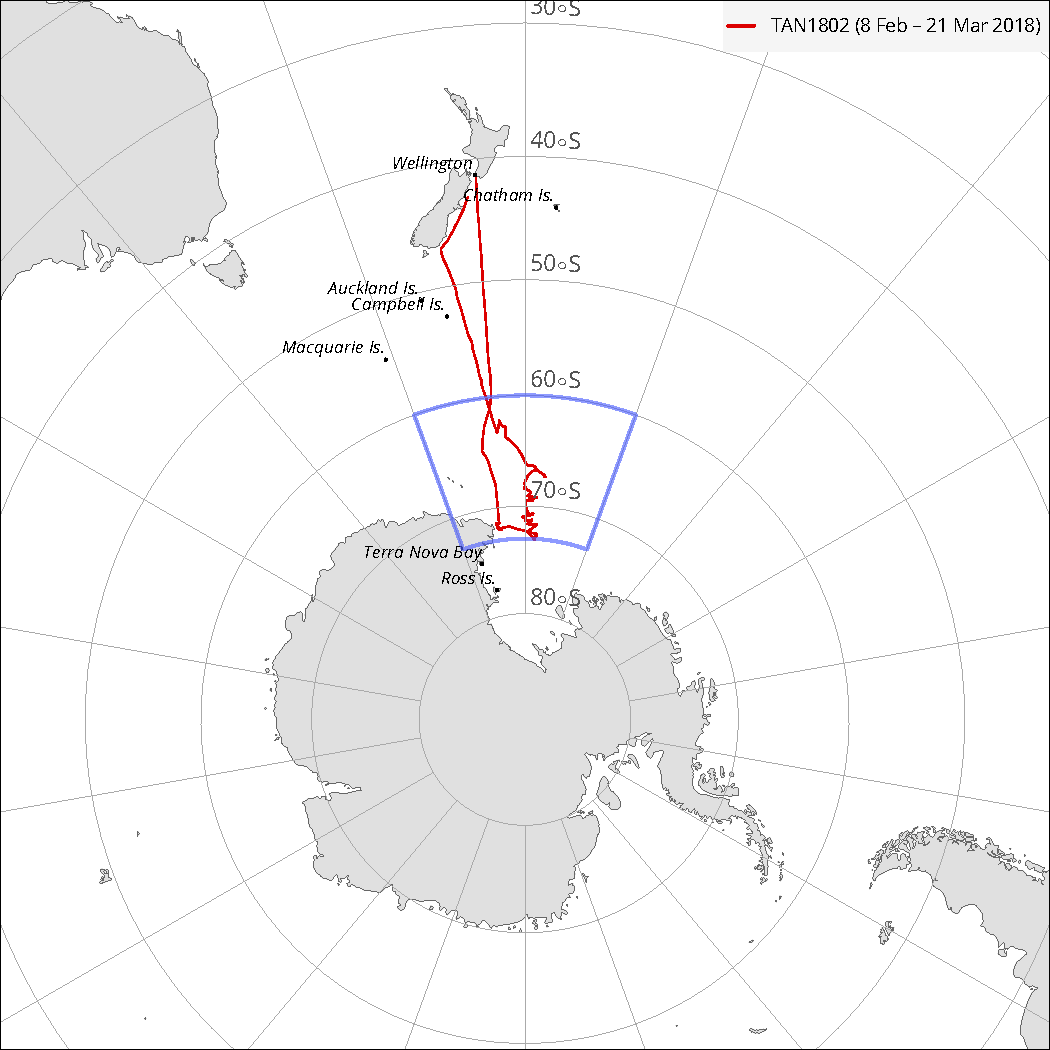
\includegraphics[width=0.5\textwidth]{img/map.pdf}
\caption{A map showing the track of the TAN1802 voyage and the region
between 60$^\circ$S and 73$^\circ$S of the TAN1802 ceilometer, radiosonde
and AWS data analysed here.
}
\label{fig:map}
\end{figure}

\clearpage

\begin{figure}[t]
%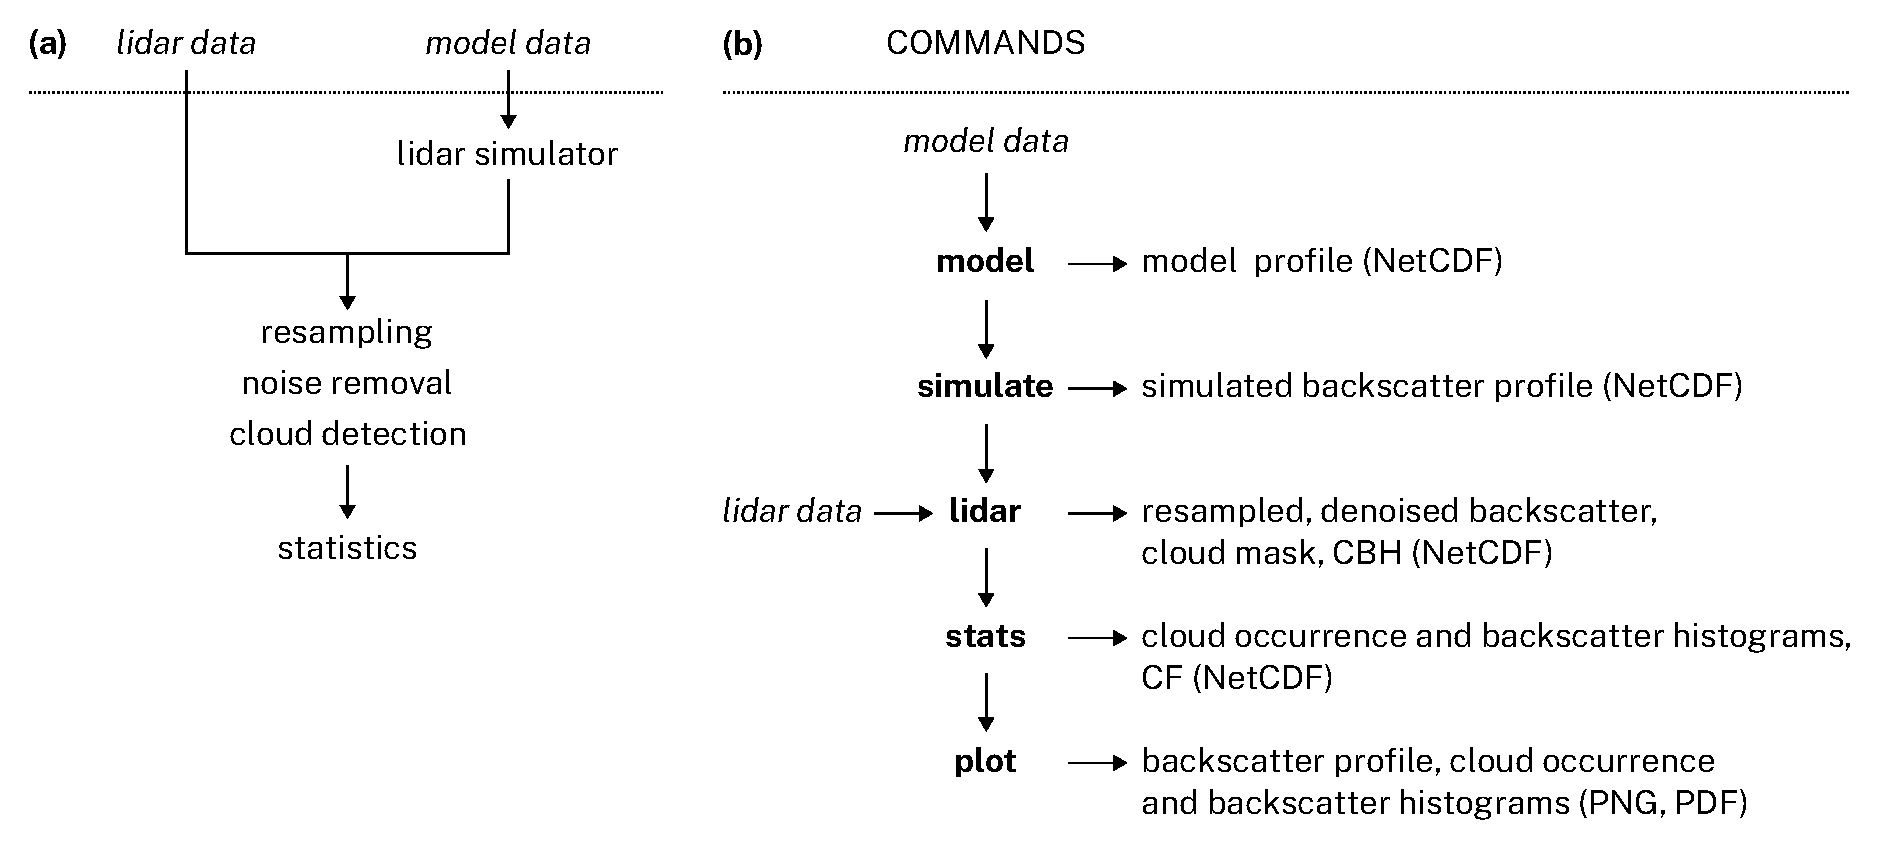
\includegraphics[width=0.7\textwidth]{img/scheme.pdf}
\caption{A scheme showing the operation of the boundary layer (BL)
and convection schemes in a cumulus (Cu) below stratocumulus (Sc) profile
commonly observed in the summertime Southern Ocean. Surface mixed layer (SML),
lifting condensation level (LCL).
}
\label{fig:scheme}
\end{figure}

\clearpage

\begin{figure}[t]
%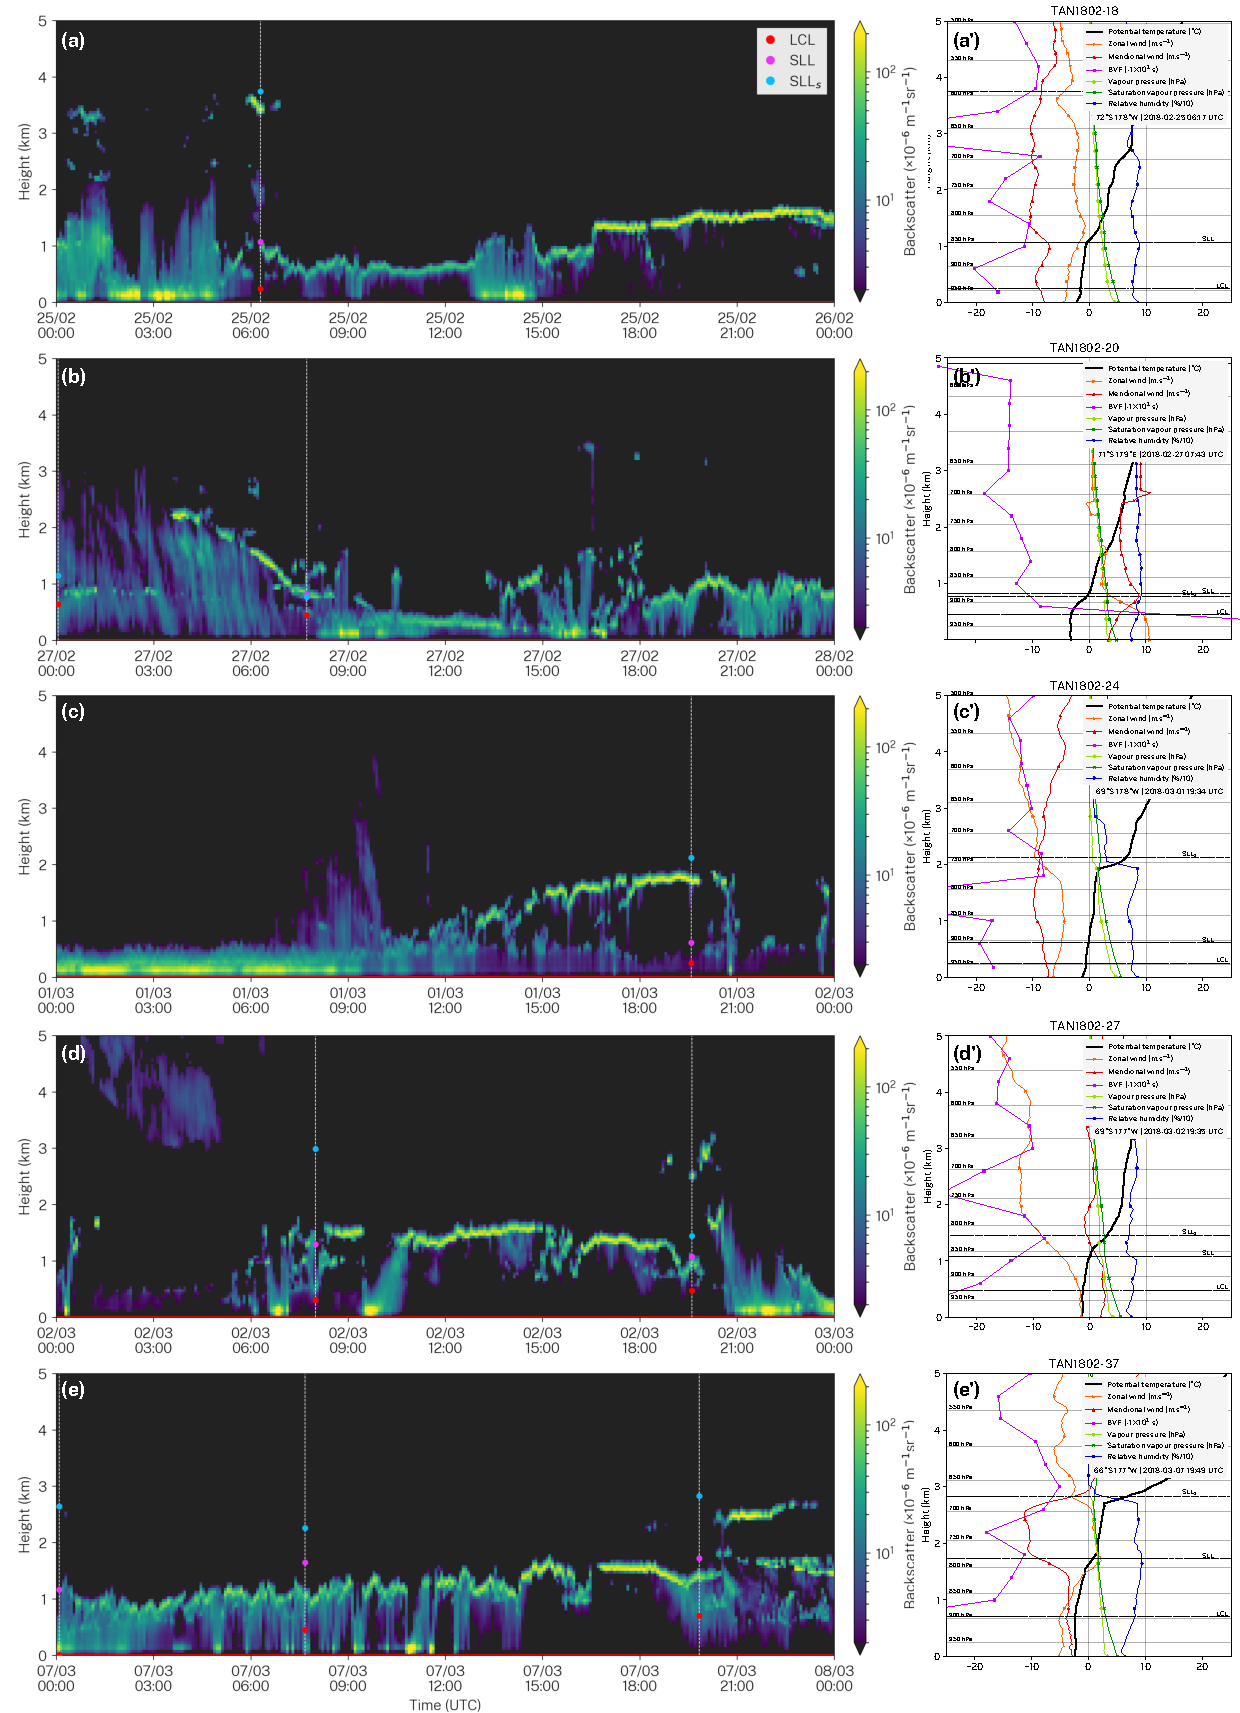
\includegraphics[width=0.75\textwidth]{img/backscatter_rs.pdf}
\caption{Selected daily backscatter profiles collected on the TAN1802 voyage
and radiosonde profiles. Shown are lifting condensation level (LCL),
SST lifting level (SLL) and SST lifting level for a saturated parcel (SLL$_s$).
Radiosonde launch times are indicated by a vertical line on the backscatter
plots and the height of LCL, SLL and SLL$_s$ is indicated by a coloured dot.
}
\label{fig:backscatter-rs}
\end{figure}

\clearpage

\begin{figure}[t]
%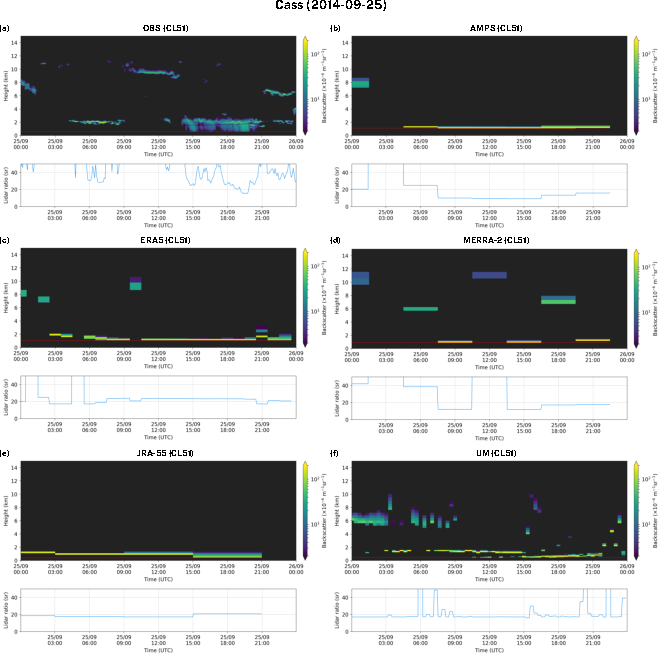
\includegraphics[width=\textwidth]{img/examples.pdf}
\caption{Selected daily observed and simulated backscatter profile plots.
The observations (OBS) were collected on the TAN1802 voyage and the
simulations are based on the UM11.4 control (UM11.4cnt) and experimental (UM11.4exp) runs
at the same time and geographical location as corresponding the observations.
The plots also show radiosonde lifting condensation level (LCL), SST lifting level (SLL), saturated SST lifting level (SSL$_s$), the model LCL, diagnostic parcel height (z$_{par}$) and
updraft detrainment rate (DTRU). The vertical extent is limited to 5 km ASL.
}
\label{fig:examples}
\end{figure}

\clearpage

\begin{figure}[t]
%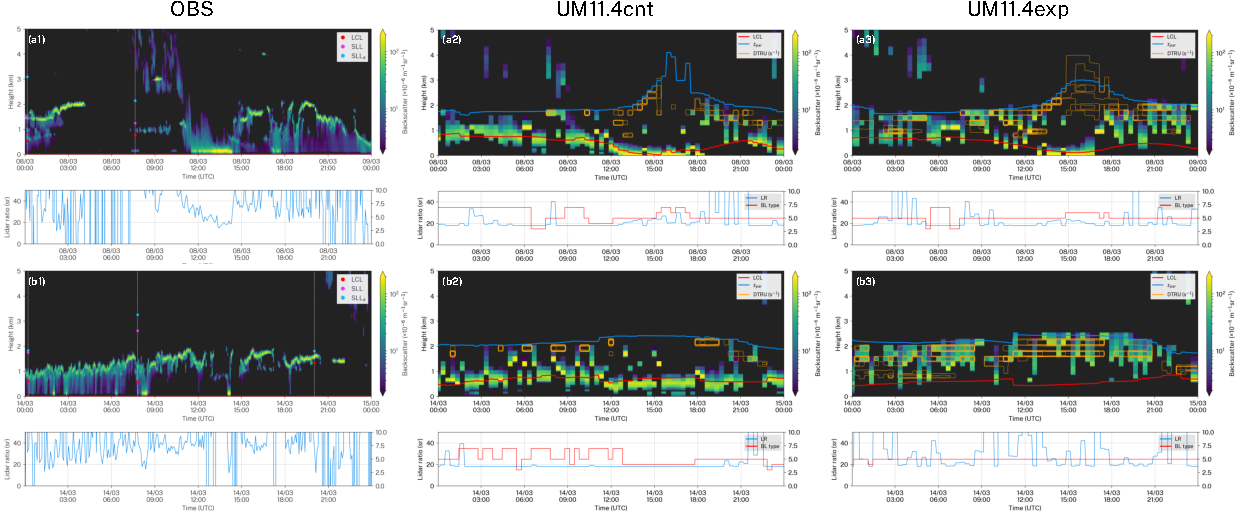
\includegraphics[width=\textwidth]{img/examples_cont.pdf}
\caption{Figure \ref{fig:examples} continued.
}
\label{fig:examples-cont}
\end{figure}

\clearpage

\begin{figure}[t]
%\includegraphics[width=0.85\textwidth]{img/examples_hur_mcu.pdf}
\caption{Mass flux (odd rows) and relative humidity (even rows) profiles in the UM11.4 control (UM11.4cnt)
and experimental (UM11.4exp) runs, corresponding to the plots in Fig. \ref{fig:examples}.
}
\label{fig:examples-hur-mcu}
\end{figure}

\clearpage

\begin{figure}[t]
%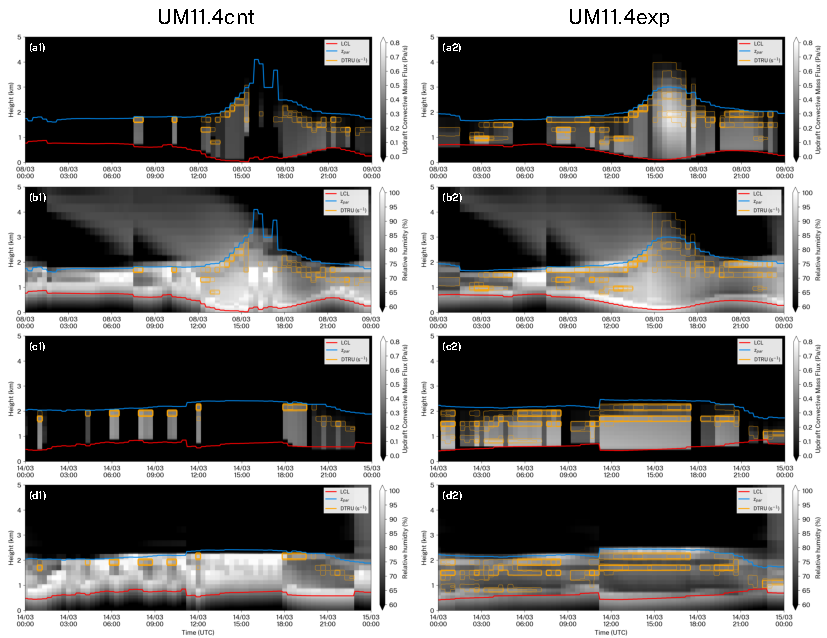
\includegraphics[width=0.85\textwidth]{img/examples_hur_mcu_cont.pdf}
\caption{Figure \ref{fig:examples-hur-mcu} continued.
}
\label{fig:examples-hur-mcu-cont}
\end{figure}

\clearpage

\begin{figure}[t]
%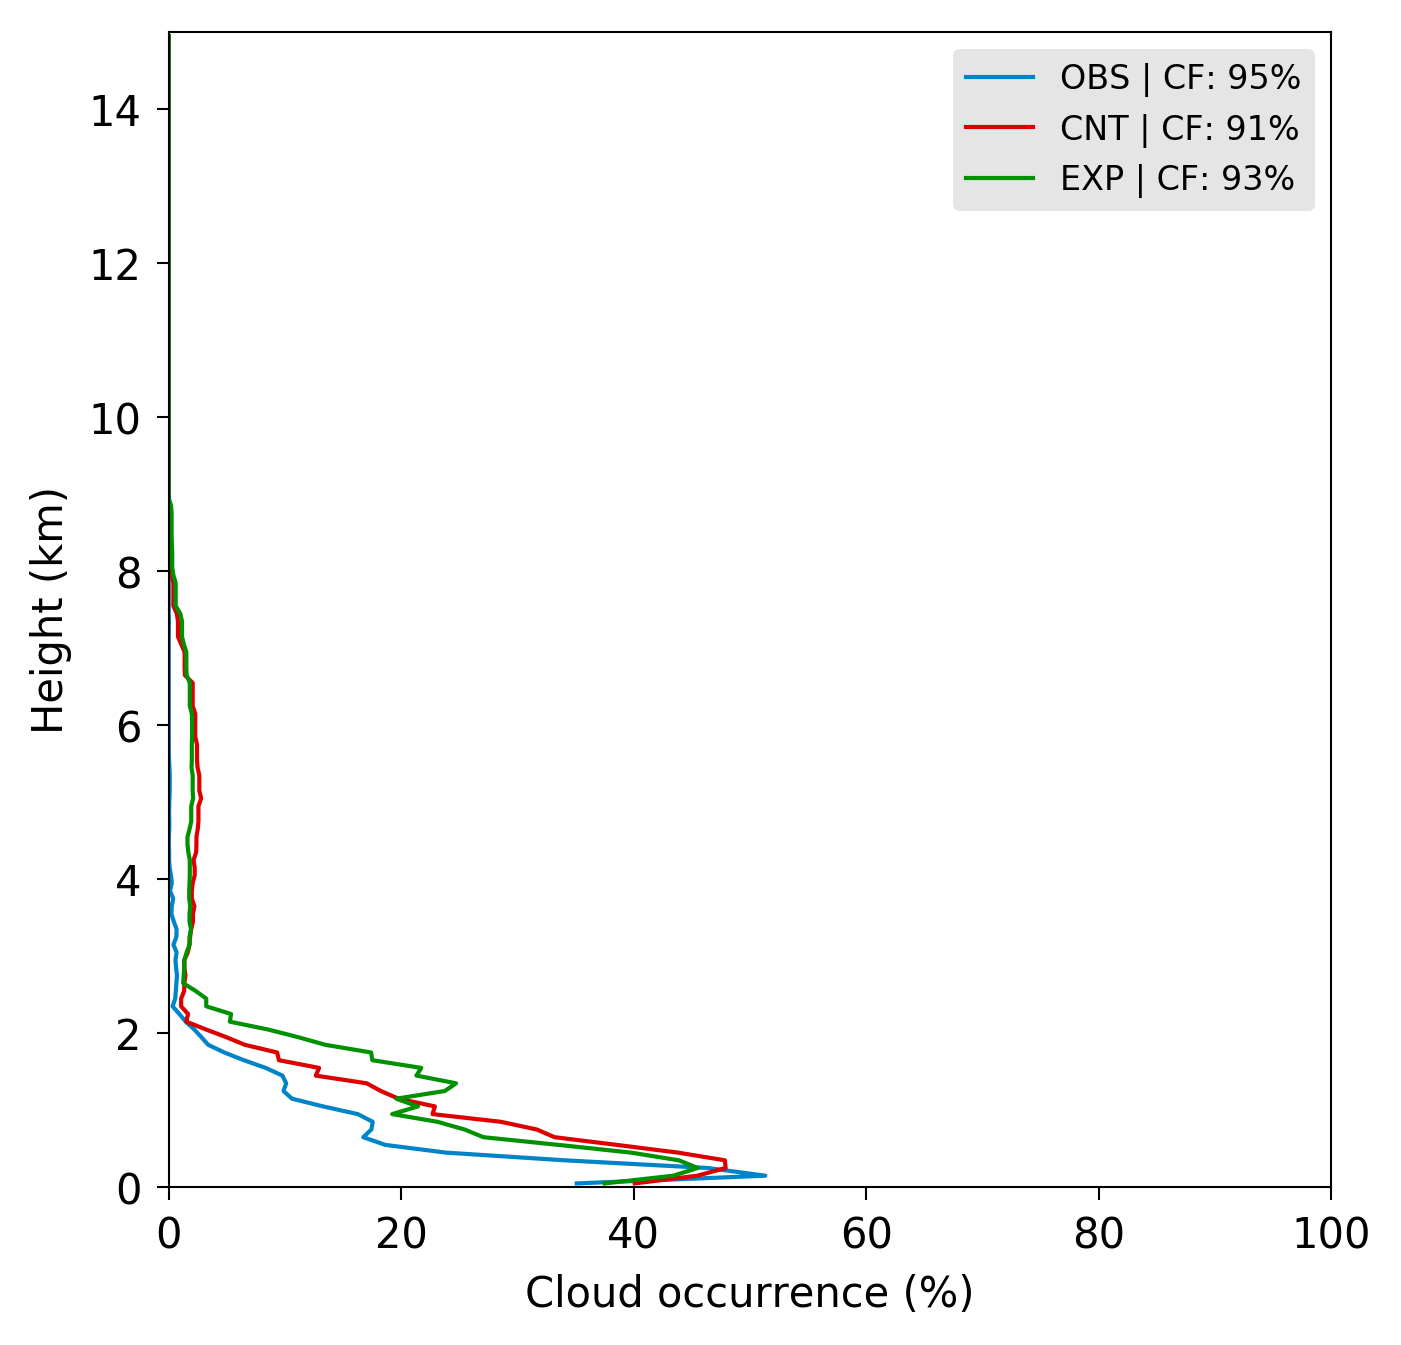
\includegraphics[width=0.5\textwidth]{img/cloud_occurrence.png}
\caption{
Cloud occurrence histogram as a function of height calculated from
28 days of the TAN1802 voyage calculated from ceilometer observations (OBS),
simulated lidar data in the control run of the UM11.4 (CNT) and
the experimental run of the UM11.4 (EXP).
Shown is also the total cloud fraction.
}
\label{fig:cloud-occurrence}
\end{figure}

\clearpage

\begin{figure}[t]
%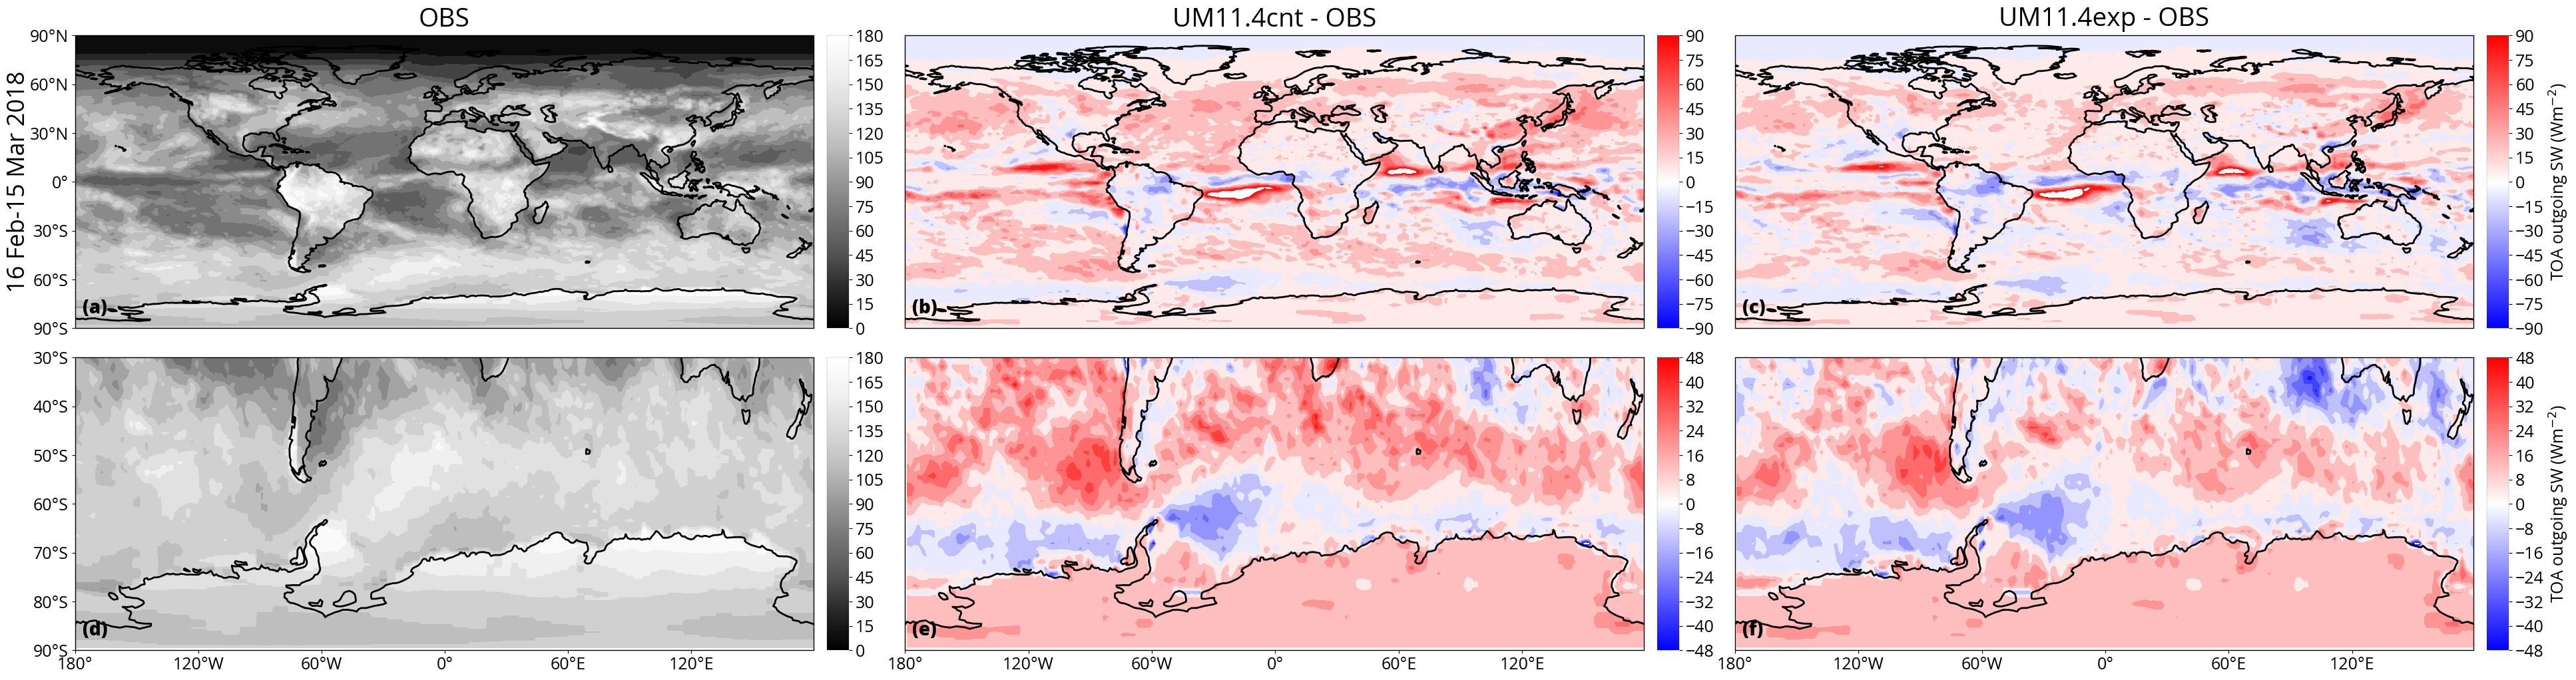
\includegraphics[width=\textwidth]{img/sw.png}
\caption{Top of atmosphere outgoing shortwave radiation in CERES SYN (OBS) and
bias in the UM11.4 control (UM11.4cnt) and experimental (UM11.4exp) runs relative
to CERES SYN during the period of TAN1802 observations 16 February--15 March 2018.
\textbf{(a, d)} show absolute values and \textbf{(b, c, e, f)} show values relative
to CERES SYN. The top row \textbf{(a--c)} shows the whole globe, the bottom
row \textbf{(d--f)} shows the Southern Ocean specifically.
}
\label{fig:sw}
\end{figure}

\clearpage

\begin{figure}[t]
%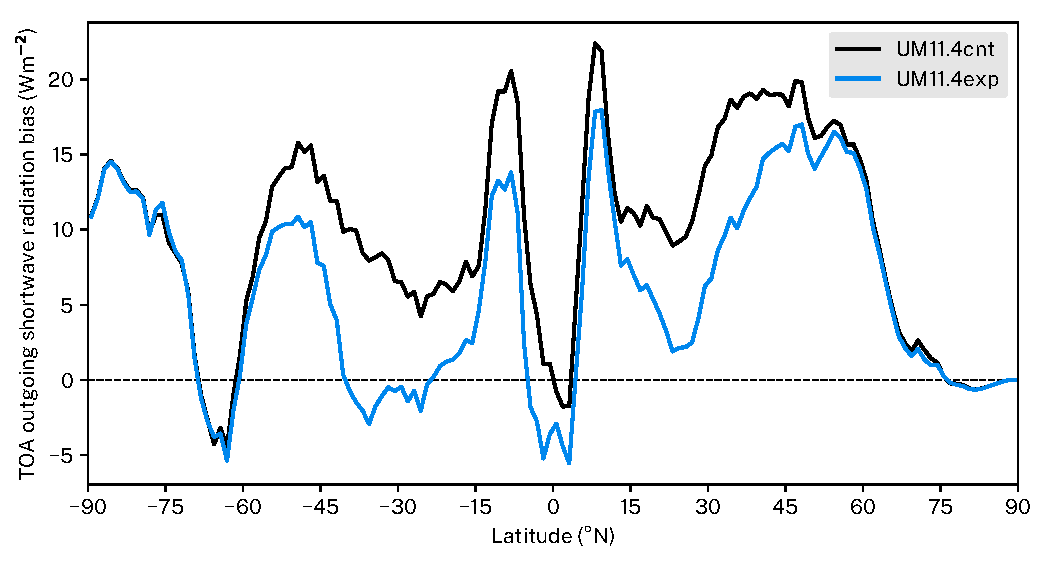
\includegraphics[width=0.75\textwidth]{img/sw_zonal.pdf}
\caption{
Zonal average of top of atmosphere outgoing shortwave radiation in
the UM11.4 control (UM11.4cnt) and experimental (UM11.4exp) runs relative
to CERES SYN during the period of TAN1802 observations 16 February--15 March 2018. 
}
\label{fig:sw-zonal}
\end{figure}

\clearpage


\begin{figure}[t]
%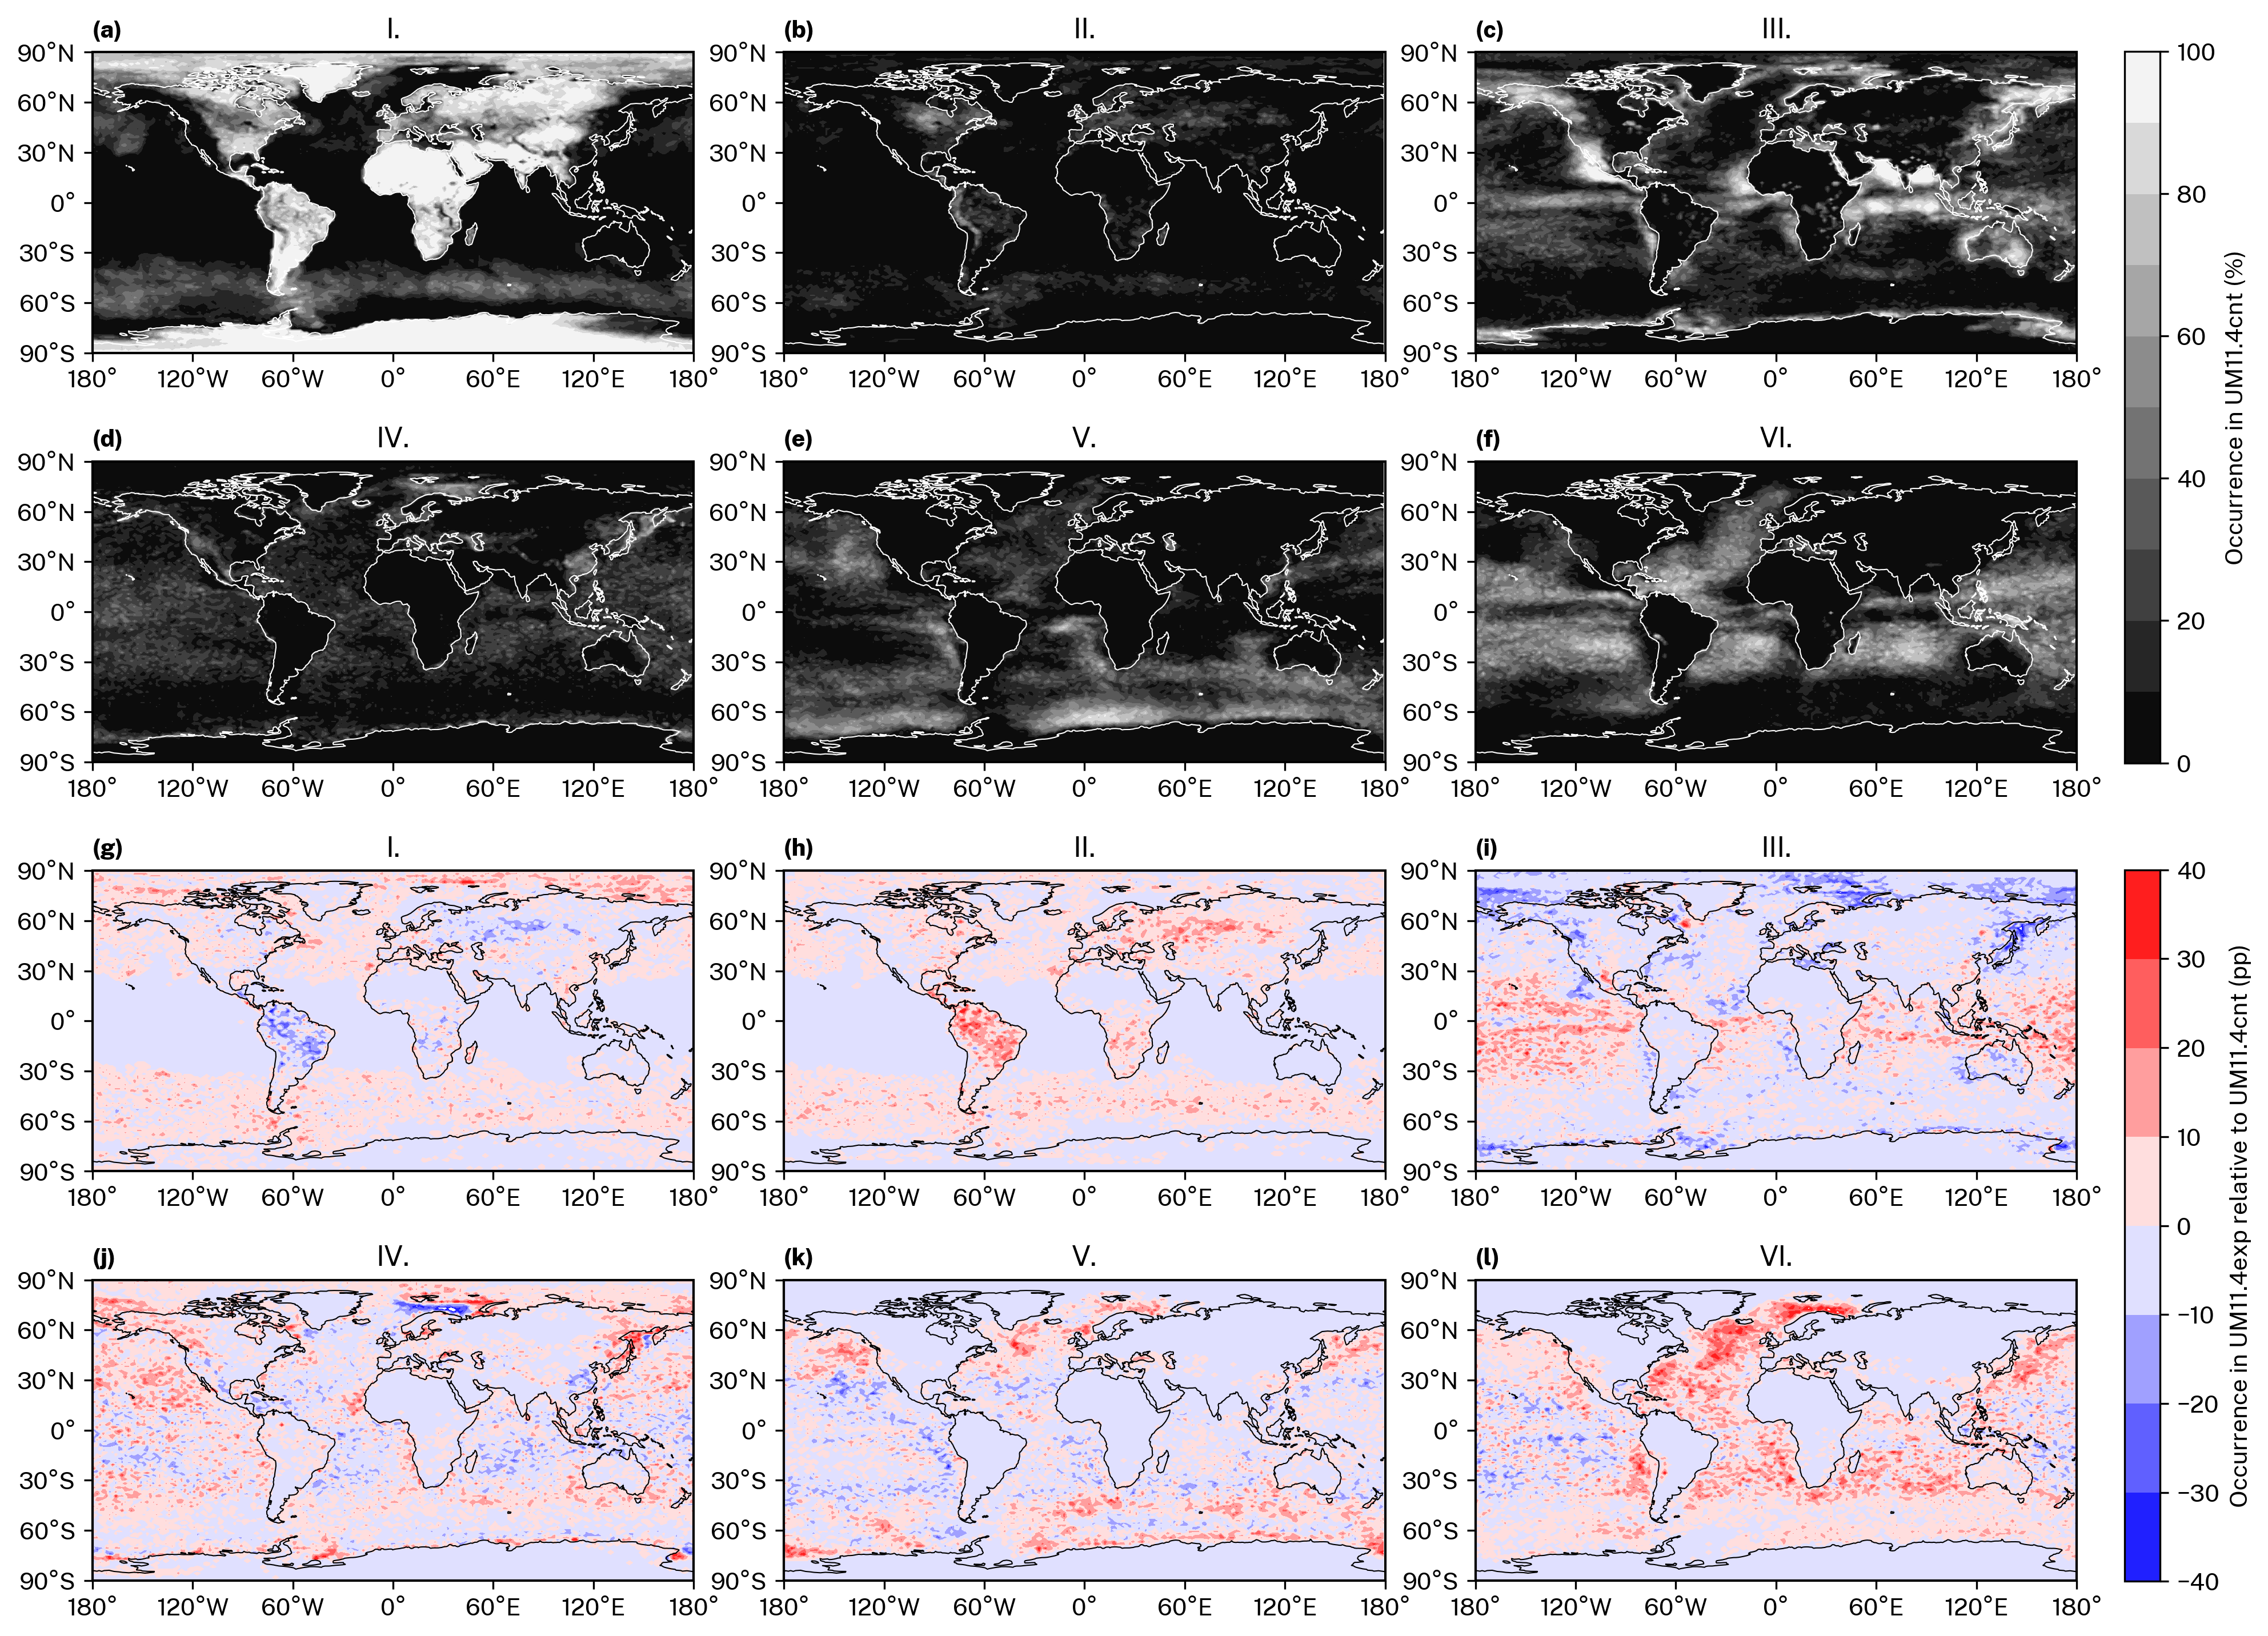
\includegraphics[width=\textwidth]{img/bdyt.png}
\caption{Boundary layer type histograms of types I.--VI. \citep{lock2000} in the UM11.4cnt
\textbf{(a--f)} and UM11.4exp relative to the UM11.4cnt \textbf{(g--l)} expressed as percentage point (pp)
difference.
}
\label{fig:bdyt}
\end{figure}

\clearpage

\begin{table}
\caption{
Summary of the cloud-related subgrid-scale parametrisations in the UM11.4.
}
\label{tab:parametrisations}
\begin{tabular}{lll}
%\tophline
Parametrisation & Principle & References\\
%\middlehline
Convection scheme & Mass flux with CAPE or surface buoyancy flux closure. & \cite{gregory1990}\\
& & \cite{grant1999}\\
& & \cite{grant2001}\\
Boundary layer scheme & First-order closure turbulence. &\cite{lock2000}\\
& & \cite{martin2000}\\
Large-scale cloud scheme (PC2) & Prognostic cloud liquid and ice. & \cite{wilson2008a,wilson2008b}\\
JULES surface flux parametrisation & The COARE algorithm. & \cite{fairall2003}\\
%\bottomhline
\end{tabular}
\end{table}

\begin{table}
\caption{
Diagnostic model levels and layers relevant to shallow boundary layer convection, turbulence
and cloud, listed from the lowest to the highest.
}
\label{tab:levels}
\begin{tabular}{llllllll}
%\tophline
Level & Description\\
%\middlehline
SL (surface layer) & Layer between the surface and the lower of 0.1$z_h$ and level where $\theta_{vl}$ starts to increase with height.\\
SML (surface mixed layer) & Turbulently well-mixed layer between the surface and LCL.\\
LCL (lifting condensation level) & Traditional definition (e.g. \cite{wallace2006}).\\
$z_h$ & Level equal to LCL if cumulus-capped, or $z_{par}$ if not.\\
$z_{par}$ & Top of a diagnostic moist parcel ascent.\\
%\bottomhline
\end{tabular}
\end{table}

